% report.tex
%
% Solving exercise 3.
% Version: alpha
%
% Copyright 2010, Lukas Prokop

\documentclass[12pt,a4paper]{article}

% PACKAGES
\usepackage[utf8]{inputenc}
\usepackage{ngerman}
\usepackage{bibgerm}
\usepackage{lmodern}

\usepackage{amssymb}
\usepackage{amsmath}
\usepackage{amsthm}
\usepackage{textcomp}
\usepackage{wasysym} % diameter

\usepackage[sf]{titlesec}
\usepackage{fullpage}
\usepackage{booktabs}
\usepackage{fancyhdr}

\usepackage[dvips,pdftex,left=2.5cm,right=2cm,
    top=1.5cm,bottom=7cm]{geometry}
\usepackage{graphicx}
\usepackage{pstricks}
\usepackage{pst-node}
\usepackage{pst-plot}

\usepackage[unicode,pdfborder={0 0 0}]{hyperref}
\usepackage{lastpage}
\usepackage{units}
\usepackage{wrapfig}

\pagenumbering{arabic}
\pagestyle{fancy}
\setcounter{tocdepth}{2}
\parindent0mm
\parskip2mm
\headheight0mm
\headsep10mm
\setlength{\unitlength}{1cm}
\setlength{\belowcaptionskip}{-30pt}

\setlength{\oddsidemargin}{0cm}
\setlength{\evensidemargin}{0cm}
\setlength{\topmargin}{0cm}

\newcommand{\ra}{\rightarrow}
\newcommand{\Ra}{\Rightarrow}
\newcommand{\la}{\leftarrow}
\newcommand{\La}{\Leftarrow}
\newcommand{\lra}{\Leftrightarrow}
\newcommand{\average}{\diameter}

\fancyhf{}


% foreign word explained; eg. \fwex{computer vision} (Maschinelles Sehen)
\newcommand{\fwex}[1]{\textit{#1}}
% foreign word; eg. \fw{computer vision}
\newcommand{\fw}[1]{\textit{#1}}
% variable for "page #"
\newcommand{\Se}[1]{S. #1}
% variable for "Abb. #"
\newcommand{\fig}[1]{Abb. #1}


\lfoot{\Se{\thepage}}
\lhead{EWA -- From the Human Eye to Computer Vision}
\rfoot{\textsc{Lukas Prokop \#1031367, Andreas Fauler \#1031225}}
\rhead{}
\renewcommand{\footrulewidth}{0.4pt}

\title{
    \Large{From the Human Eye to Computer Vision} \\
    \small{Einführung in das wissenschaftliche Arbeiten} \\
    Betreuer Dipl.-Ing. Mauthner Thomas \\
    \footnotesize{Sprache: Deutsch}
}
\author{
    Lukas Prokop \# 1031367 \\
    Andreas Fauler \# 1031225 \\
    \small{\texttt{\{lukas.prokop,fauler\} @ student.tugraz.at}}
}
\date{\today}

\begin{document}

% ''To suppose that the eye, with all its inimitable contrivances for
% adjusting the focus to different distances, for admitting different
% amounts of light, and for the correction of spherical and chromatic
% aberration, could have formed by natural selection, seems, I freely
% confess, absurd in the highest degree possible.''

% -- Charles Darwin, On the Origin of Species by Means of Natural
% Selection, or the Preservation of Favoured Races in the Struggle for
% Life, Bantam Books, 1999 (reprint of 1859 original), 155.
\maketitle
\tableofcontents

\newpage

\begin{abstract}
  In dieser Arbeit setzen wir uns mit dem Auge als Medium für die
  visuelle Wahrnehmung auseinander. Der Mensch nimmt visuelle
  Eindrücke auf, vergleicht sie unwillkürlich mit Erfahrungswerten
  und trifft Entscheidungen auf Basis derer. Der Bereich der \fw{computer
  vision} ist daran interessiert das Auge technisch nachzubauen,
  um die digital-visuelle Wahrnehmung zu ermöglichen. Dieser
  Bericht setzt sich mit der Funktionsweise der Bildverarbeitung
  im menschlichen Körper von der Hornhaut über die Netzhaut bis
  zum Visuellen Cortex auseinander, um Ausblick auf technische
  Nachbauten zu geben.
  Kameratechnologien und \fw{smartsensors} sind heute Teil unseres
  technischen Alltags und implementierte Bildverarbeitungsalgorithmen
  und Sensortechniken basieren auf dem natürlichen Vorbild.
\end{abstract}

\section{Biologische Aspekte des Auges}

Das Auge ist jenes Sinnesorgan der Lebenswesen, welches für die visuelle
Wahrnehmung und damit Interpretation von Lichtsignalen zuständig ist. Das
menschliche Auge kann Lichtwellen im Bereich von \unit[350]{nm} bis zu
\unit[750]{nm} wahrnehmen. Diese Signale werden an der Netzhaut gespiegelt
abgebildet, von Stäbchen und Zapfen in elektromagnetische Reize umgewandelt
und im Gehirn verarbeitet. Diese Informationen nutzt der Mensch, um seine
Umgebung zu beobachten und damit überlebensfähig zu bleiben
\cite{sensorarray}.

Die Augen liegen symmetrisch in den Augenhöhlen beider Gesichtshälften,
wodurch das menschliche Augenpaar frontal angeordnet ist, wie es bei allen
Jägern in der Natur vorkommt. Es ist an die verschiedenen natürlichen
Lebensweisen des Menschen angepasst. So kann ein gesunder Mensch sehr gut
Farbsehen, bewegliche Objekte verfolgen und durch kontrastreiches Sehen
Konturen und Helligkeiten unterscheiden. Durch die Elastizität der Linse
und das Anspannen der \fwex{Corpus ciliare} (Zonulafasern) kann er nahe und
ferne Objekt fokusieren, um sie scharf erkennen zu können. Diese Anpassung
der Linse an die Entfernung nennt sich \fwex{Akkomodation}. Jedoch ist der
Mensch nicht in der Lage (wie es bei Vögeln der Fall ist), Objekte in
einem beschränkten Bereich der \fwex{Retina} (Netzhaut) stark vergrößert
zu sehen. Das Auge des Menschen ist wie bei den meisten Wirbeltieren als
physiologisch hoch entwickelt einzustufen \cite[\Se{58}]{anatomie}.

Diese biologischen Gegegebenheiten sind jedoch nicht mehr an unsere
heutigen Lebensgewohnheiten angepasst. Wir beschränken uns im Alltag auf
das Fokusieren von nahen Objekten (Zeitung lesen, Arbeit mit Bildschirmen),
weshalb es oft zur Volkskrankheit Sehschwäche in Form von Kurz- oder
Weitsichtigkeit kommt.

\subsection{Der anatomische Aufbau des Auges}
\label{sec:ana}

\begin{figure}[!h]
  \begin{center}
    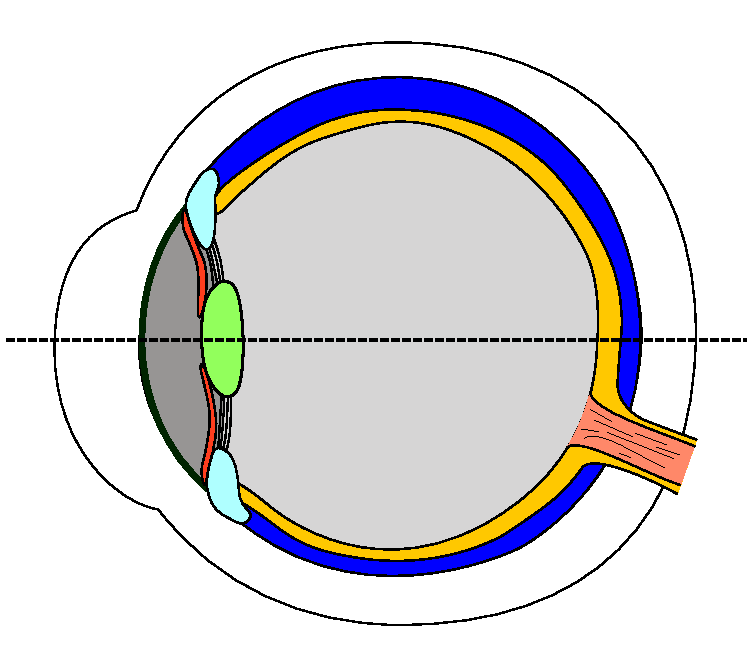
\includegraphics[scale=0.7]{imgs/eye.pdf}
    \caption[Querschnitt des menschlichen Auges]
        {\emph{Aufbau des menschlichen Auges.} Bestehend aus Lederhaut (weiß),
        Aderhaut (blau), Netzhaut (orange), Sehnerv (salmon), Ziliarmuskeln
        (türkis), Zonulafasern (schwarze Linien), Linse (grün), Iris (rot),
        Hornhaut (dunkelgrün), hintere Augenkammer (hellgrau), vordere
        Augenkammer (dunkelgrau)}
    \label{img:human_eye}
  \end{center}
\end{figure}

Das Auge befindet sich in der Augenhöhle des Skeletts und wird von einer
undurchsichtigen, weißlichen Lederhaut umgeben. Das Licht dringt entlang
der Sehachse durch die Hornhaut. Zwischen Hornhaut und Linse befindet sich
die vordere Augenkammer. Die Linse wird abgedeckt durch die Regenbogenhaut
(Iris) und die Pupille. Die Linse funktioniert wie ein Fotoapparat und
bricht die Lichtstrahlen, sodass sie vertikal gespiegelt auf der Netzhaut
abgebildet werden.

Die Sehachse trifft an der Netzhaut auf den Gelben
Fleck; der ein Zentrum scharfen Sehens bildet. Umgekehrt wird der Bereich
an dem der Sehnerv auf die Netzhaut trifft, als Blinder Fleck bezeichnet,
da der Mensch an dieser Stelle nichts erkennen kann. Allerdings bemerkt ein
gesunder Mensch diesen Fleck nicht, da das zweite Auge diesen Fleck
ausgleicht und das Gehirn fehlende Flächen im Bild mit künstlichen Farben
ergänzt.

Schützen kann sich das Auge durch das Zusammenziehen der Iris. Dadurch fällt
weniger Licht in den Glaskörper (Innere des Auges). Gegen physikalische
Gefahren können sich die Lider ausfalten und damit die gesamte Augenoberfläche
abdecken. Die Lider haben auch die Funktion die Hornhaut feucht zu halten,
damit das Auge durch die großen Augenmuskeln beliebig gedreht werden kann
ohne Reibungserscheinungen auftreten zu lassen. Die Tränenflüssigkeit
wird in den Tränendrüsen gebildet
%% zu genau
%und mit Ausscheidungen der Meibomschen
%Drüsen vermengt, wodurch sie verdunstungsresistenter wird. Zusätzlich
%befinden sich die Ausgänge der Moll-Drüsen an den Wimpern, die keimtötende
%Substanzen abgeben
und reinigt das Auge, wenn Partikel unter das Augenlid kommen \cite{anatomie}.

\subsection{Die Retina als bildgebender Sensor}

%% Edited by Andy. Siehe Absatz ''Die Retina (Netzhaut) besteht''
%Trifft das Licht auf die Netzhaut, wird es von verschiedenen Arten von
%Nervenzellen interpretiert. Die fotorezeptiven Zellen umfassen die Zäpfchen
%und Stäbchen sowie weitere Zellarten. Die Interneurone und Ganglienzellen
%leiten die Signale an Nervenbahnen außerhalb des Augapfels weiter.
%Interessant sind besonders die kegelförmigen Zäpfchen und zylinderähnlichen
%Stäbchen. Während Erstere für das Farbsehen zuständig sind, empfangen
%zweitere insbesondere schwache, reduzierte Signale (skotopische Anpassung).
%Die Zäpfchen umfassen dabei 3 verschiedene Zapfenformen: rot-, grün und
%blauempflindliche. Folglich gibt es Zäpfchen die auf Licht verschiedener
%Wellenlängen reagieren (rot als sehr langwelliges Licht und blauviolett
%ist kurzwellig). Durch das Vorhandensein dieser drei Typen, kann das
%komplette Farbspektrum abgebildet werden (RGB-Farbmodell).

Die Retina (Netzhaut) besteht grob unterteilt aus drei
Schichten von Nervenzellen. In der obersten Schicht befinden sich
lichtempfindliche Zellen, sg. Fotorezeptoren \cite{retinapathways}.

\begin{figure}[p]
  \begin{center}
    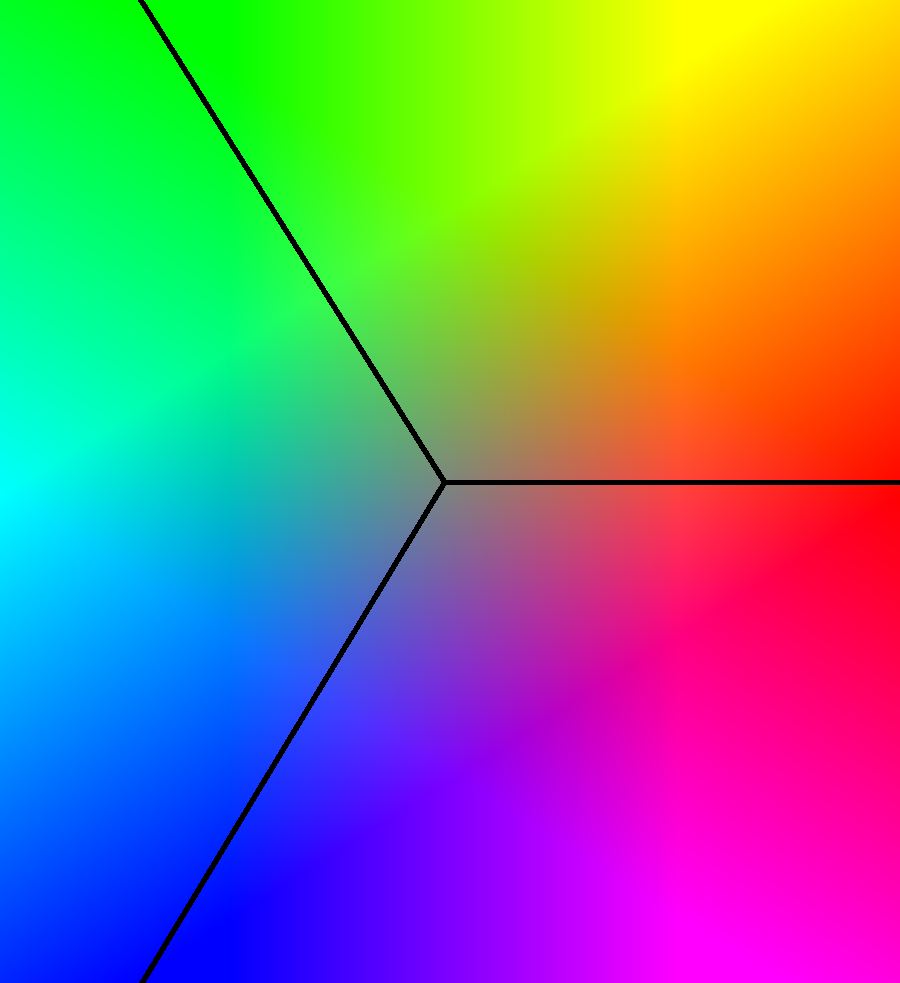
\includegraphics[width=0.2\textwidth]{imgs/rgb.pdf}
    \caption
     [modifizierter Screenshot der RGB Farbauswahl aus dem Grafikprogramm GIMP]
     {Das RGB Farbspektrum. Entlang der schwarzen Linien befinden sich
      die drei additiven Farben Rot Grün Blau. Weitere Farben ergeben sich
      durch das Mischen dieser drei Grundfarben.}
    \label{img:rgb}
  \end{center}
\end{figure}

Trifft das Licht auf die Netzhaut, wird es von diesen Rezeptoren interpretiert.
Die fotorezeptiven Zellen umfassen die Zäpfchen und Stäbchen sowie weitere
Zellarten. Interessant sind besonders die kegelförmigen Zäpfchen und
zylinderähnlichen Stäbchen. Während erstere für das Farb- und das detailreiche,
scharfe Sehen zuständig sind, empfangen zweitere insbesondere schwache,
reduzierte Signale. So sind die Stäbchen für das Sehen bei geringer Helligkeit
und in den Randlagen der Netzhaut zuständig. Die Zäpfchen umfassen drei
verschiedene Zapfenarten: rot-, grün und blauempflindliche. Folglich gibt es
Zäpfchen die auf Licht verschiedener Wellenlängen reagieren (rot
repräsentiert sehr langwelliges Licht, während blauviolett kurzwellig
ist). Durch das Vorhandensein dieser drei Typen kann das komplette Farbspektrum
abgebildet werden (RGB-Farbmodell, \fig{\ref{img:rgb}}). Die Stäbchen \&
Zäpfchen verursachen eine Teilung der Informationen Farben und Helligkeit.
Dabei handelt es sich um ein Konzept, welches 1:1 in die Bionik übernommen
wurde.

Der Unterschied zwischen den verschiedenen Aufgabengebieten (scharfes bzw.
peripheres Sehen) ergibt sich teilweise durch die Ungleichverteilung der
Rezeptorzellen auf der Netzhaut. So befinden sich im Zentrum -- beim Gelben
Fleck -- viele Zäpfchen dicht bei einander, während in der Peripherie die
Dichtheit der Zellen (hauptsächlich Stäbchen) wesentlich kleiner ist.
Am Gelben Fleck kann man etwa 50 000 Ganglienzellen pro Quadratmillimeter
beobachten, während sich in der Peripherie nur etwa 1000 Zellen pro
Quadratmillimeter finden lassen. Unter der Annahme, dass der Radius des
Augapfels eines ausgewachsenen Menschen etwa 12mm beträgt und der Gelbe
Fleck etwa 2$^\circ$ in Anspruch nimmt, so beträgt die Fläche des Gelben
Flecks (unter Vernachlässigung der Krümmung) etwa \unit[$1.7013^{-5}$]{$mm^2$}.
So ergibt sich zwar ein kleineres scharfes Sichtfeld, die Menge an eingehender
Information und damit der Aufwand bei der Verarbeitung ist aber wesentlich
geringer. Aus dem Grund der besseren Sichtbarkeit entlang der Sehachse bewegt
der Mensch seinen Kopf jeweils in die für ihn interessante (bzw.
aufmerksamkeitserregende) Richtung, wobei das Sehfeld des Menschen etwa
$130^\circ$ vertikal und $180^\circ$ horizontal umfasst.

\subsection{Das neurowissenschaftliche Modell des Retinaaufbaus}

Betrachten wir die Retina im Detail, gibt es verschiedene Modelle, um die
Interaktion der Synapsen\footnote{Kontaktschnittstelle zwischen 2 Zellen}
zu beschreiben. Im Folgenden sei das neurowissenschaftliche Modell erklärt,
welches sich an der Aufgabenverteilung der Zellen orientiert.

\newpage
\begin{wrapfigure}{r}{0.4\textwidth}
  \begin{center}
    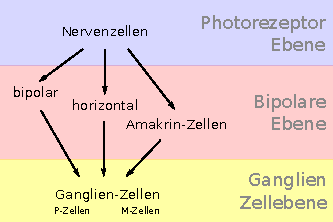
\includegraphics{imgs/layers_without_gradients.pdf}
    \caption[Die Ebenen der vertikalen Signalleitung]
        {Die Ebenen der vertikalen Signalleitung. Symbolisch
        würden unter der Ganglien-Zellebene Nervenbahnen zum Gehirn
        liegen.}
    \label{img:layers}
  \end{center}
\end{wrapfigure}

Die oberste Schicht von Nervenzellen leitet die Signale an die darunterliegende
Schicht weiter. In dieser befinden sich bipolare Zellen, horizontale Zellen
und auch Amakrin-Zellen (\fig{\ref{img:layers}}). Aufgrund der -- verglichen
mit den Fotorezeptorzellen -- geringeren Anzahl dieser Zellen ist eine Zelle
für mehrere, verschiedene Rezeptorzellen der oberen Ebene ''zuständig''.
Daraus ergibt sich für jede Zelle ein sg. rezeptives Feld, also ein Bereich
aus dem diese Zelle Signale erhält. Die bipolaren und horizontalen Zellen
haben entgegengesetzte Aufgaben. Während die bipolaren Zellen bei einem Reiz
im Zentrum des rezeptiven Felds Signale weiterleiten, übernehmen die
horizontalen Zellen Reize die am Rand ihres zugeteilten Feldes auftreten. Die
Amakrin-Zellen \cite[\Se{2}]{retinapathways} steuern den Umfang der rezeptiven
Felder und die Stärke der Reaktion auf Reize innerhalb dieser. Sie sind
wesentlich für Aufgaben wie Bewegungserkennung, Konturenwahrnehmung und
Helligkeitsanpassung. Man hat 22 verschiedene Unterarten von Amarkin-Zellen
entdeckt. Zwischen all diesen Zellarten gibt es über die Ebenen synaptische
Verbindungen, die Datenströme erlauben \cite{vim}.

Die unterste Schicht bilden Ganglien-Zellen. Sie sind die Schnittstelle
zwischen der Retina und dem Gehirn. Hier werden die Signale schlussendlich
über den Sehnerv an das Gehirn weitergereicht. Nachdem das Verhältnis von
Fotorezeptoren und Ganglienzellen über 100:1 beträgt
\cite[\Se{4}]{retinapathways} müssen die Informationen vor dem Transport noch
''komprimiert'' werden, was teilweise schon in der zweiten Schicht
geschehen ist. Grundsätzlich unterscheidet man zwei\footnote{Man nimmt an,
dass es etwa 12-15 verschiedene Subtypen von Ganglienzellen gibt} Typen von
Ganglienzellen: P-Zellen (für parvozellular) und M-Zellen (magnozellular),
\cite[\Se{4}, \Se{1}]{retinapathways} wobei die P-Zellen 90\% aller
Ganglien-Zellen ausmachen und vor allem im Zentrum der Retina vorkommen.
Auch die Ganglien haben rezeptive Felder, das heißt auch hier ist eine Zelle
für viele Rezeptoren ''zuständig'' (das ergibt sich schon aus der großen
Überzahl an Rezeptorzellen). Die rezeptiven Felder sind im Gelben Fleck sehr
klein, d.h. die Ganglien sind nur für sehr wenige (bzw. einzelne)
Rezeptorzellen zuständig, während nach außen hin die rezeptiven Felder groß
werden. Außerdem haben M-Zellen stets größere rezeptive Felder als P-Zellen.

Von den P- und M-Zellen gehen korrespondierende P- und M-Leitungen aus, über
welche die Informationen schließlich über Nervenbahnen in das Gehirn
transportiert werden. Im Sinne des neurowissenschaftlichen Modells haben
die P-Zellen das Ziel, möglichst verlustfrei zu arbeiten und somit möglichst
\emph{viele} Daten an das Gehirn weiterzuleiten. Deshalb kommt es zur
besagten Komprimierung der Daten. Umgekehrt haben M-Zellen das Bestreben
die Daten möglichst \emph{schnell} an das Gehirn weiterzuleiten \cite{vim}.

\section{Von der Retina zur Bildverarbeitung}
\label{sec:rebi}

Visuelle Reize werden im hinteren Teil des Großgehirns verarbeitet; im
sogenannten Okzipitallappen. Dieser besitzt das primäre und sekundäre
Sehzentrum, die gemeinsam den Visuellen Cortex (VC) bilden. Während
sich das primäre Sehzentrum um die Aufnahme der Informationen (sowohl
jeder Bildpunkt wird interpretiert als auch Linien und Konturen aus dem
Gesamtbild separat gefiltert) kümmert, so übernimmt das sekundäre Sehzentrum
die Aufgabe des Abgleichs mit Erfahrungswerten und Erinnerungen. Allgemein
bekannt ist, dass es zu einer kontralokalen Relation kommt: Die \emph{linke}
Gesichtshälfte nimmt Informationen für die \emph{rechte} Gehirnhälfte auf.

%\begin{wrapfigure}{l}{0.5\textwidth}
\begin{figure}[p]
  \begin{center}
    
\includegraphics[width=0.4\textwidth]{imgs/optical_illusion.png}
    \caption
      [
       ''Optische Täuschung'' unter der GNU FDL lizensiert.
       Zuletzt abgerufen am 12. Dezember 2010 14:15 \hspace{15pt}
       \url{http://www.dailycognition.com/content/image/14/800px-cafe-wall.png}
      ]
      {
       Beispiel einer optischen Täuschung. Es kommt zu einer
       Fehlinterpretation der Daten im sekundären Sehzentrum, da das
       Gehirn gewohnt ist, versetzte Objekte in eine Tiefenrelation
       zu setzen.
      }
    \label{img:illusion}
  \end{center}
\end{figure}
%\end{wrapfigure}

Hirnforscher teilen den visuellen Cortex in 5 Bereiche auf. Während der
Begriff des primären Sehsystems mit dem primären Bereich (V1) übereinstimmt,
ist das sekundäre Sehsystem in V2--V5 aufgeteilt.

Erwähnt sei hier noch der LGN. Der \fwex{Lateral geniculate nucleus}
(Metathalamus) ist ein subkortikaler Vorbereich des Visuellen Cortex,
der eine Filterfunktion besitzt und die Aufgabe hat, Informationen an den
geeigneten Bereich des VCs weiterzuleiten. Allerdings werden die meisten
Daten direkt an den V1 gesandt. Er empfängt die Daten der Retina von der
Sehbahn (Nervenbahnen vom primären zum sekundären Sehsystem) und reicht
sie an den V1 weiter. Der LGN besteht aus sechsfach geschichteten
Zellenschichten, wobei M- und P-Zellen im Verhältnis 2:4 auf diesen
Schichten aufgetragen sind. Die M- und P-Zellen unterscheiden sich in
der oben erwähnen räumlichen Dichte und dem Aufbau ihrer Fortsätze
(Dendriten). Die P-Zellen besitzen kleine Dendrite und damit haben sie
ein hohes Auflösungsvermögen. Sie erlauben das Farbsehen. Die M-Zellen
hingegen bilden wieder einen Gegenpol der Bilddaten von der Retina und
verarbeiten mit ihrem wesentlich größeren rezeptiven Feld Helligkeitsstufen
\cite{vim}.

Wir erwähnten, dass die Retina mit einem RGB-Farbmodell arbeitet. Dieses zieht
sich bis zum LGN vollständig durch (\fig{\ref{img:rgb_reaction}}). Allerdings
gibt es auch einen Hemmungsfaktor für das RGB-Farbmodell. Wird eine Zelle
durch die Farbe rot erregt, kann diese durch grünes Licht gehemmt werden.
Selbiges gilt für die Farben Blau zu Gelb. Welche Relevanz dieses
Gegenfarbmuster für die Verarbeitung und Weiterleitung der Sinnesempfindungen
hat, ist noch nicht eindeutig geklärt.

\begin{figure}[h]
  \begin{center}
    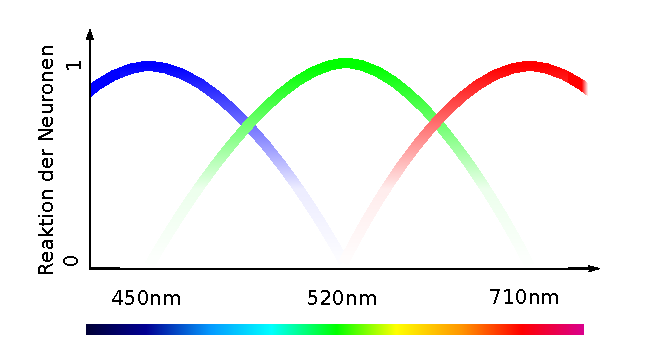
\includegraphics[width=0.4\textwidth]{imgs/rgb_neuronal_reaction.pdf}
    \caption[Reaktionsverhalten der Neuronen auf RGB-Farben]
     {Die Grafik illustriert das Reaktionsverhalten der Neuronen
      auf RGB-Farben. Wird grüne Farbe empfangen, werden nur Neuronen der
      Farbe Grün aktiviert. Wird Türkis empfangen, werden sowohl grüne
      als auch blaue Neuronen erregt.}
    \label{img:rgb_reaction}
  \end{center}
\end{figure}

Bei einem erheblichen Schaden der M-Zell-Schichten im LGN lassen sich klare
Beeinträchtigungen im Bewegungssehen beobachten, während ein Schaden der
P-Zell-Schichten eine zerstörte Tiefen-, Struktur- und Farbwahrnehmung
hervorrufen \cite{schiller}.

\subsection{Das Brodmann-Areal 17, die Area striata oder der V1}

Beim V1 handelt es sich um den best erforschtesten Teil des VC. Die
\fwex{fMRI}-Technologie (functional magnetic resonance imaging) (eine
Unterklasse der MRIs) hat hier wesentliche Beiträge geleistet. Sie erlaubt
einen visuellen Einblick in die neuronalen Aktivitäten im Verhältnis zum
zeitgleichen Blutfluss. Letzterer spielt eine wesentliche Rolle bei der
funktionellen Arbeit der Neuronen, da bei neuronaler Reaktion die Zelle
sofort Glukose anfordert, um den entsprechenden Energiebedarf zu befriedigen
und regt damit auch den Blutstrom an \cite{brainactivation}.

Im V1 werden die Informationen vom LGN empfangen. Man vermutet, dass die
Informationen einer Verarbeitung hierarchischer Ordnung unterliegen. Man kann
generell festlegen, dass die Bilddaten von V1 bis V5 weitergereicht werden
und stufenweise verarbeitet werden. Dies lässt sich beobachten, weil das
rezeptive Feld Ebene für Ebene immer größer wird, sodass die
Bildinformationen in den höheren Ebenen kontextsensitiver verarbeitet werden
können als im V1. Grundsätzlich gibt es 2 Datenströme, die die Bilddaten in
die höheren kortikalen Bereiche bringen: der vorderseitige Datenstrom
(V1 $\ra$ V2 $\ra$ V5 $\ra$ Parietallappen) und der rückseitige Strom
(V1 $\ra$ V2 $\ra$ V3 $\ra$ V4 $\ra$ Temporallappen). Es ist allerdings sehr
schwer diese beiden Ströme entlang des Visuellen Cortex zu verfolgen, da
Daten oftmals über getrennte, kortikale Kanäle übertragen werden (als
Beispiel sei hier die Farb- \& Helligkeitsseparation erwähnt). Zu diesem
Ergebnis kamen auch Yoshinobu Goto, Takao Yamasaki und Shozo Tobimatsu in
ihrer Arbeit \cite{retinapathways} in der sie zusammenfassend erwähnen, dass
die physikalische Natur von visuellen Stimulationen von mehreren, separaten
und parallelen Leitungen auf mehreren Seiten im Sehsystem getragen wird.

Gewisse Neuronenklassen im V1 reagieren bevorzugt auf einfache Reize wie Linien
einheitlicher Richtung in einem beschränkten Gesichtsfeld. Umgekehrt reagieren
Neuronenklassen des V5 auf Gesamtbilder wie Gesichter und Hände unabhängig von
ihrer Position im Gesichtsfeld und ihrer Drehung.

Die Neuronen im LGN und V1 sind anatomisch und funktional in 2 Bereiche
getrennt, die separat Form (Objekterkennungsaufgaben) und Bewegung
(Objektortung -- Bewegungsrichtung und räumliche Position) verarbeiten,
obwohl jeweils Verbindungsstellen zwischen den beiden Bereichen existieren
\cite[\Se{2}]{arch}. Im V1 konnte 3 verschiedene Arten von Neuronen
nachgewiesen werden: einfache Neuronen, komplexe Neuronen und hyperkomplexe
Neuronen \cite{hubel}, die sich alle im Detail für unterschiedliche Bilddaten
interessieren. Genauso kann man aber eine Einteilung der Neuronen in die 3
Gruppen vornehmen, die sensitiv für Farben, die Position des Objekts oder
eine Mischung aus beiden sind.

Die Daten werden im V1 \fw{retinotop} abgebildet. Die Retinotopie bezeichnet
den Effekt der neuronalen Reaktion beim Betrachtens einer Form: Betrachtet
man eine Form, wird eine Neuronenaktivität im VC hervorgerufrn, die die
selbe Form hat. Retinotopie in dieser Art kommt bei allen Primaten vor.

Die neuronalen Netze im V1 unterscheiden sich durch Erwartungswerte bezüglich
der Eingabeparameter, ihrer internen Verschaltungen (ähnlich Logikgattern)
und ihrem Antwortverhalten. Zum Beispiel kann es Unterschiede geben wie
Antworten aufgebaut sind (fixe Größen gegenüber einem Datenstrom). Das selbe
Verhalten wurde 1:1 für \fwex{FIR}-Filter (finite impulse response)
übernommen.

Weil sich die enorme Dichte an Informationen an der enormen Dichte an
neuronalen Netzen widerspiegelt, wird der V1 illustrativ auch als
''\fwex{Sortierbüro}'' (sorting office) bezeichnet.

\subsection{Die Reaktionen des V1 auf visuelle Stimulation am Beispiel
    eines Experiments}

2004 wurden Experimente an den japanischen Universitäten Tokai University
und Waseda University durchgeführt, wie das Gehirn auf Reize reagiert.
Die Reaktionen des V1 wurden mit der fMRI-Technik
aufgezeichnet \cite{brainactivation}.

\subsubsection{Ein Quadrat als Reiz}

Die Versuchsperson befindet sich in einem abgeschotteten Raum und wird
mit visuellen Reizen auseinander gesetzt. Sie sieht frontal auf einen
Bildschirm. Auch wenn die Forscher auch mit auditiven Reizen experimentieren,
beschäftigt sich das erste Experiment nur mit Eindrücke im Sehsystem.
Ein quadratisches Muster wächst um die Größe von \unit[110]{\%} alle
\unit[750]{ms} an. Diese Größenveränderung geschieht 2mal pro
Versuchsdurchlauf.

\emph{Ergebnis:} Der Visuelle Cortex wurde bei allen Versuchspersonen
vollständig aktiviert. Wie erwartet konnte die Größe des Musters direkt an
der neuronalen Aktivität abgelesen werden (die Neuronenaktivität ist direkt
proportional zur Größe des Musters). Die Bereiche des Temporallappens wurden
ebenso von den visuellen Eindrücken stimuliert. Allerdings war der VC
wesentlich stärker belastet als der Temporallappen. Bereiche des
nahegelegenen Hörsystems wurden nicht genutzt.

Die untersuchenden Physiologen kommen zu dem Schluss, dass dynamische Reize
(sowohl sich visuell verändernde Reize als auch visuelle und Audioreize, die
versetzt auftreten) die einzelnen Cortex stärker aktivieren als statische
Wahrnehmungen. Aus diesem Experiment geht hervor, dass das Gehirn für
unveränderte Informationen nur geringfügige Kapazitäten vergibt.

Des Weiteren interessiert die Wissenschaftler die Korrelation zwischen
verschiedenen Reizen unterschiedlicher Quellen. Als Beispiel sei erwähnt,
dass wir auf Basis von einer gesehenen Form und einem erfahrenen Geschmack
diese Form auf den Geschmack abbilden können und diese beiden Reize
zukünftig assoziieren. Welche physiologischen und psychologischen Modelle
darauf gründen, ist noch ungewiss \cite{brainactivation}.

\section{Die Bionische Umsetzung}

\subsection{Offene Fragen}

Es sind noch offene Fragen in der Physiologie des menschlichen Auges vorhanden.
So gilt der V1 als gut erforscht, doch über die höheren Ebenen des Visuellen
Cortex ist wenig bekannt. Genauso wurde in dieser Arbeit verschiedene
doppelseitige Datenströme vorgestellt (Helligkeitsfaktor und RGB-Farben,
vorderseitiger und rückseitiger Datenstrom, \dots). Es ist allerdings unklar,
welche Relevanz diese Ströme wirklich besitzen und in welcher Form die Daten
folglich im Gehirn gespeichert werden. Es kann kein eindeutiger Schluss auf die
Datenverarbeitung gemacht werden und die technischen Implementierungen nutzen
meist eigene Konzepte, die sich an technischen Gegebenheiten orientieren
\cite{arch}.

Retinamodelle, die direkt von den Erkenntnissen der Neurowissenschaft umgesetzt
werden, werden mit Problemen des Energieverbrauchs, der Echtzeitsimulation,
der Zuverlässigkeit, der Augapfeldrehung zur Verfolgung von Objekten und der
Chipgröße konfrontiert \cite{retinapathways}. Mathematische Konzepte zur
Sehachsenausrichtung sind in der Arbeit von B.W. Lin und Ou Ma
\cite{modanalysis} einsehbar.

\subsection{Verarbeitungsgeschwindigkeit}

Eindrucksvoll konnte das Team rund um Simon Thorpe \cite{thorpe} die
Verarbeitungsgeschwindigkeit des V1 feststellen. Es gab viele Fragen bezüglich
der Geschwindigkeit, da Daten, die zwischen V1 und V5 übertragen wurden,
meist nur wenige Schaltstationen passieren. Danach wurde der Kontext der
Bilddaten vollständig aufgelöst und Entscheidungen werden bereits getroffen.

Die Probanden sahen Bilder mit natürlichen Szenen, die mit einer bestimmten
Wahrscheinlichkeit Tiere enthielten. Der Proband wurde ersucht eine Taste
zu drücken, solange kein Tier gesehen werden konnte. Nach der Auswertung
der Versuchsreihe stellte Simon Thorpe et al. fest, dass es bis zum Lösen
der Taste durchschnittlich nur 300 Millisekunden dauert. Inbegriffen in
dieser Zeit sind selbstverständlich die Zeit der Übertragung der
Bildinformation ins Gehirn als auch die motorische Reaktionsfähigkeit.
In einem weiteren Versuchsaufbau wurden die neuronalen Reaktionen mit einem
\fwex{Elektroenzephalogramm} (EEG) gemessen. Fazit dieser empirischen
Untersuchung war es, dass bereits nach 150 Millisekunden das Gehirn sein
Urteil gefällt hat, wobei noch etwa 70 Millisekunden für den Transport
der Daten in den primären Sehbereich zu subtrahieren sind. Folglich
schafft es das Gehirn in etwa 80 Millisekunden ein Urteil zu fällen;
eine Zeitspanne, die nach Modellen bisheriger Experten nicht erreicht
werden konnte.

\subsection{Die technische Implementierung in Bildsensoren}

Das dem menschlichen Sehapparat zugrundeliegende Prinzip findet sich im Groben
auch in digitalen Kameras. Was für das Auge die Retina ist, sind für digitale
Kameras die Bildsensoren. Sie wandeln das einfallende Licht in elektrische
Signale um.
Es gibt verschiedene Arten von Bildsensoren, am gebräuchlichsten sind CMOS-
(Complementary Metal Oxide Semiconductor) und CCD-Chips (Charge-Coupled
Device) \cite{photo}. Obwohl bei beiden Sensorarten die eintreffenden
Photonen (Lichtteilchen) elektrische Ladungen generieren, unterscheiden
sie sich in einigen Punkten.

Vereinfacht gesagt, besteht ein CCD-Chip \cite[\Se{1}]{photo} unter anderem
aus einer zweidimensionalen, rechteckigen Anordnung von Kondensatoren
(vorstellbar als Gitter oder Tabelle). Im lichtsensiblen Teil werden die
einfallenden Photonen über eine bestimme Zeit gesammelt und so eine Ladung
generiert. Diese Ladungspakete werden dann von Kondensator zu Kondensator
weitergegeben. Dabei wird die Schranke zwischen zwei Kondensatoren
durchlässig, sodass die Ladungen weiterwandern können. So wandern die
Ladungen der obersten Zelle jeder Spalte nach unten. Dort befindet sich ein
gemeinsamer Ausgabe-Verstärker für alle Spalten.
Diese Konfiguration bedingt, dass die Bildinformationen aller Pixel zur exakt
gleichen Zeit gesammelt werden. Außerdem bedingt die Verwendung einer
gemeinsamen Ausgabestufe, dass diese bei hoher Pixelanzahl und
Bildwiederholraten mit hoher Frequenz arbeiten muss.

Bei CMOS-Chips \cite[\Se{2}]{photo} hingegen ist jeder Pixel einzeln
ansprechbar. Die jeweilige Sensorzelle beendet, wenn sie elektronisch
angesprochen wird, die Sammlung von Photonen und gibt die entsprechende
Ladung an einen eigenen Verstärker weiter. Nach dieser ''Entleerung'' kann
die Sensorzelle sofort wieder mit dem Sammeln von Lichtteilchen beginnen.
Vor der nächsten Entladung werden alle anderen Sensorzellen entleert.
Dieses Funktionsprinzip bedingt, dass die Bildinformationen aller Pixel zu
unterschiedlichen Zeiten gesammelt werden. Dadurch, dass jeder Pixel seine
eigene Ausgabestufe hat, können diese auch bei hohen Auflösungen und
Bildwiederholraten mit geringeren Frequenzen arbeiten.

Diese unterschiedlichen Funktionsweisen bedingen verschiedene Vor- und
Nachteile \cite{photo}. Dadurch dass CCD-Sensoren beispielsweise nur einen
Ausgabeverstärker benutzen, ist der Anteil an Rauschen im Verhältnis zum
Bildsignal (\fw{signal-to-noise-ratio}) wesentlich geringer. Allerdings wirkt
sich diese Bauform bei Anwendungen wo Geschwindigkeit bzw. eine hohe
Bildwiederholrate ein Kriterium sind (z.B. Video) negativ aus.

Neben der Anwendung bei digitalen Videokameras finden sich CMOS-Chips vor allem
im Consumer-Bereich (z.B. in Mobiltelefonen). Das liegt neben dem geringeren
Preis bei der Herstellung auch daran, dass CMOS-Chips weniger Strom verbrauchen
und geringere Spannungswerte zum Funktionieren benötigen.

Beide Sensorarten haben sich in den letzten Jahren aber in ihren Eigenschaften
angeglichen \cite[\Se{6}]{compis}.

\subsection{Der Ausblick}

Trotz der offenen Fragen, widersprüchlichen Modelle und technischen
Schwierigkeiten kann man von einem wesentlichen Fortschritt der Bionik auf
diesem Gebiet sprechen; die letzten Jahre haben die \fw{computer vision}
grundlegend verändert. Kameras sind in jedem Handy enthalten und Sensoren
entscheiden über unseren Komfort in Autos. Die Zukunft ist gesichert; nicht
zuletzt aufgrund des wirtschaftlichen Interesses zuverlässige, digitale Augen
zu produzieren und auch des allgemeinen Interesses des Menschen seine eigene
Funktionsweise zu verstehen.

% http://en.wikipedia.org/wiki/Visual_system
% http://verficktescheisse.com/how-its-done-glass-eye/
% Rudich, Andreas: Automatische Kartierung der Retina (1996)
% Bernoegger, Stefan: Kartierung der menschlichen Retina (1997)
% http://de.wikipedia.org/wiki/Kategorie:Physiologie_des_Auges
% http://en.wikipedia.org/wiki/Image_sensor

\newpage

\listoffigures

Graphiken ohne Lizenz unterstehen der
\href{http://www.gnu.org/licenses/fdl.html}{GNU FDL} (Free Documentation
License) und wurden mit dem freien Grafikprogramm
\href{http://inkscape.org/}{Inkscape} erstellt.

\bibliographystyle{plain}
\bibliography{report}

\end{document}
